
\taskpic{ Верёвка длиной $l$ закреплена одним из своих концов в
  вершине сферы радиуса $R$. В некоторый момент верёвку
  отпускают. Найдите ускорение верёвки сразу после этого. Трение
  отсутствует.   }
{
  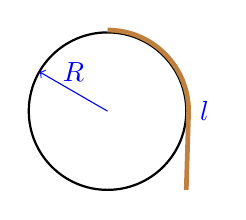
\begin{tikzpicture}
    \draw[thick] (2,2) circle (1cm);
    \draw[line width=0.06cm,brown] (2,3.03) arc (90:0:1.03cm)
    node[right,blue] {$l$};
    \draw[line width=0.06cm,brown] (3.03,2) -- (3,1);
    \draw[->,blue] (2,2) -- ++(150:1cm) node[midway,above] {$R$};
  \end{tikzpicture}
}
% Квант, Ф1273, 1991-6
